\documentclass[11pt,a4paper]{article}
\usepackage[a4paper,hmargin=1in,vmargin=1in]{geometry}
\usepackage{pgfplots}
\pgfplotsset{compat=1.17}

\usepackage[czech]{babel}
\usepackage[utf8]{inputenc}
\usepackage[T1]{fontenc}

\usepackage{stddoc}
\usepackage{lipsum}
\usepackage{subcaption}

\newcommand{\plus}{{\texttt{+}}}
\renewcommand{\Re}{\operatorname{Re}}
\renewcommand{\Im}{\operatorname{Im}}
\newcommand{\fourier}[3]{\mathcal{F}_{#1}\!\left[#2\right]\!\left(#3\right)}
\newcommand{\ifourier}[3]{\mathcal{F}^{-1}_{#1}\!\left[#2\right]\!\left(#3\right)}

%--------------------------------------------------------------------
% Package amsthm setup
%--------------------------------------------------------------------
\makeatletter
\def\thmheadbrackets#1#2#3{%
	\thmname{#1}\thmnumber{\@ifnotempty{#1}{ }\@upn{#2}}%
	\thmnote{{ \the\thm@notefont[#3]}}}
\makeatother

\newtheoremstyle{my-theorem}	% name
{\topsep}						% Space abovetommy
{\topsep}						% Space below
{\slshape}						% Body font
{}								% Indent amount
{\bfseries}						% Theorem head font
{.}								% Punctuation after theorem head
{1em}							% Space after theorem head
{\thmheadbrackets{#1}{#2}{\bfseries#3}}	% theorem head spec

\newtheoremstyle{non-theorem}	% name
{\topsep}						% Space abovetommy
{\topsep}						% Space below
{\normalfont}					% Body font
{}								% Indent amount
{\bfseries}						% Theorem head font
{.}								% Punctuation after theorem head
{1em}							% Space after theorem head
{\thmheadbrackets{#1}{#2}{#3}}	% theorem head spec

\theoremstyle{my-theorem}
\newtheorem{theorem}{Theorem}[section]
\newtheorem{claim}[theorem]{Claim}
\newtheorem{corollary}[theorem]{Corollary}
\newtheorem{lemma}[theorem]{Lemma}
\newtheorem{proposition}[theorem]{Proposition}

\theoremstyle{non-theorem}
\newtheorem{definition}[theorem]{Definition}
\newtheorem{remark}[theorem]{Remark}
\newtheorem{example}[theorem]{Example}
\newtheorem{notation}[theorem]{Notation}
\newtheorem{note}[theorem]{Note}

\renewcommand{\qedsymbol}{$\blacksquare$}
\renewenvironment{proof}[1][\proofname]{{\scshape #1. }}{\qed}


\begin{document}

\pagenumbering{arabic}

% Header
\noindent\LARGE\textbf{RNVA přednáška - 5. týden}\normalsize\\
\noindent\rule{14.5cm}{0.4pt}

\section{Navigační systémy (dokončení z minula)}

\subsection{GLONASS}
Ruský navigační systém
\begin{itemize}
    \item 1970: zahájení vývoje
    \item 1982: první testovací družice
    \item 1996-2001: úpadek systému v důsledku ekenomických potíží Ruska
    \item 2001: začalo se s rekonstrukcí systému
\end{itemize}
Ruská technologie byla vždycky trochu crazy $\Rightarrow$ moc se jim to zezačátku nedařilo a museli to tam \uv{střílet naslepo}.

\paragraph*{Konstelace}
\begin{itemize}
    \item 24 družic
    \item 3 oběžné roviny vzájemně pootočené o $120^\circ$
    \item kruhové dráhy o inklinaci $64.8^\circ$
    \item výška 19100 km
    \item oběžná doba 11 hod 58 min
\end{itemize}

\paragraph*{Signál} 
\begin{itemize}
    \item Kmitočty L1 a L2
    \item BPSK 511 kchip/s
    \item Posloupnost maximální délky o délce 512 chipů
    \item FDMA
    \begin{align*}
        f_{k,L1} &= 1602 + 0.5625k \; \mathrm{MHz},
    \\
        f_{k,L2} &= 1201 + 0.4375k \; \mathrm{MHz},
    \end{align*}
    kde $k \in (-7, 6)$.
\end{itemize}
\begin{note} Vícero:
    \begin{itemize}
        \item Nepoužívali CDMA, ale FDMA (frekvenční multiplex), protože na to asi dřív neměli technologi digital signal processingu. Ona je posloupnost maximální délky prej ale stejně o něco lepší.
        \item Proč ne nějaký normální hodnoty $k$ jako $k = 1$ nebo tak? Ono to tak ze začátku bylo, ale to je frekvence spíš tak na radio-astronomii, takže jim to nefungovalo xD
    \end{itemize}
\end{note}

\paragraph*{Modernizace GLONASS} Nové signály s kódovým multiplexem (CDMA) na L1 a L5. Taktéž implementovali interoperabilitu s GPS a Galileo.

\subsection{Galileo}
Navigační systém EU
\begin{itemize}
    \item 1999 Evropská unie plánuje vybudovat civilní družicový navigační systém. Projekt byl financován soukromými investory.
    \item 2003 první fáze výstavby (ER, ESA)
    \item Od 2004 systém spravuje European GNSS Agency (GSA), jejíž sídlo bylo v roce 2012 přesunuto do Prahy
    \item 2006 zkrachovalo financování projektu ze soukromých zdrojů kvůli velkému riziku, a proto se v roce 2007 Evropská unie rozhodla financovat projekt z vlastních zdrojů.
    \item V roce 2005 a 2008 byly vypuštěny první testovací družice GIOVE-A a GIOVE-B.
    \item První navigační družice byly vypouštěny od roku 2011.
\end{itemize}
\begin{note}
    Galileo má pro civilní účely proklatě rychlý kód (šířka kanálu 90 MHz oproti 20 MHz u GPS). Ono to tak i začalo, že EU argumentovala tím, že svět potřebuje civilní navigační systém a že Galileo vůůůbec není navržen za jakýmikoli vojenskými účely.
\end{note}

\paragraph*{Konstelace}
\begin{itemize}
    \item 30 družic rozmístěných ve třech oběžných rovinách. Výška družic bude 32222 km a životnost 12 let.
    \item Někdy se hovoří o tom, že konstelace bude doplněna o geostacionární družice systému EGNOS.
\end{itemize}
\begin{note}
    Když hitnula hospodářská krize, tak Evropa začala s kecama jako \uv{Ono těch 30 družic, na kterých jsme trvali, vlastně neni tolik potřeba. Bude stačit třeba 17. Galileo vlastně nemá být samostatný systém, ale podpůrný systém GPS pro Evropu.}
\end{note}

\paragraph*{Signály a služby}
\begin{itemize}
    \item Galileo Open Service (OS): bezpečná služba poskytovaná na kmitočtu E1 nebo na dvou kmitočtech E1 a E5.
    \item Galileo Safety of Life Service (SOL): služba OS rozšířená o varování uživatele, že není garantována přesnost nebo integrita systému. Služba bude poskytována prostřednictvím modernizovaného systému EGNOS (EGNOS v3).
    \item Galileo Commercial Service (CS): služba bude umožňovat komerčním subjektům implementovat družicové rozšíření systému (SBAS Sattelite Based Augmentation System). Pro tuto službu bude vyhrazet zvláštní datový kanál o rychlosti 500 bps na kmitočtu E6.
    \item Galileo Public Regulated Service (PRS): služba je výhradně určena pro uživatele autorizované vládami členských států EU. Služba bude vybavena mechanizmy proti zaručení a podvrhnutí signálu. Bude sloužit k zabezpečení potřeb bezpečnostní a strategické infrastruktury jako jsou telekomunikace a finance.
\end{itemize}
\begin{note} Vícero:
    \begin{itemize}
        \item Služba PRS je vlastně taková obezlička, jak Galileo používat jako vojenský navigační systém. Nesmí se to tak ale prezentovat, takže je to pro \uv{využití vlád členských států}.
        \item Služba pátrání a záchrany Cospat-Sarsat.
    \end{itemize}
\end{note}
\begin{figure}[!ht]
    \begin{center}
        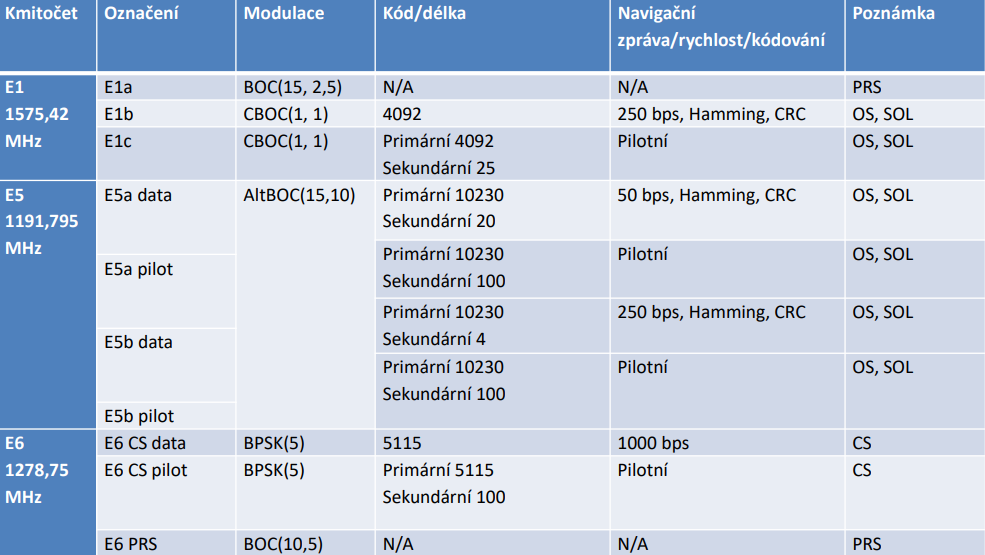
\includegraphics[width=\textwidth]{src/galileo-signals.png}
    \end{center}
    \label{fig:galileo-signals}
    \caption{Signály systému Galileo}
\end{figure}

\subsection{Compass}
Čínský navigační systém
\begin{itemize}
    \item 2000 BeiDou
    \item 2011 Compass (BeiDou-2): V témže roce disponoval 10 družicemi, které zabezpečovaly navigační službu v pacifické oblasti. Globální pokrytí je plánováno v roce 2020.
\end{itemize}
\begin{note}
    Postup implementace byl podobný jako v Evropě: Hodně se slíbilo a pak hovno z toho. Taky jim to trvalo ranec.
\end{note}
\paragraph*{Konstelace}
\begin{itemize}
    \item 3 družice na IGSO (Inclined GeoSynchronous Orbit)
    \item 27 družic na střední oběžné dráze MEO: výška 21.527 km, inklinace $55^\circ$.
\end{itemize}

\subsection{Rozšiřující navigační systémy}
Vylepšují přesnost, dostupnost a spolehlivost navigační informace. Toto je hojně využíváno například pro letectví, které má z hlediska všech tří zmíněných požadavků úplně jiné nároky než civilní sektor. Dělí se na
\begin{itemize}
    \item GBAS (Ground-Based Augmentation System)
    \item SBAS (Satellite-Based Augmentation System)
\end{itemize}
a využívají diferenční metody měření (DGNSS):
\begin{itemize}
    \item Měření se provádí ve dvou bodech: referenční stanice v bodě se známou polohou a uživatelský přijímač.
    \item Korekce korelovaných chyb (korigované DGNSS): chyba polohy a časové základny navigační družice, chyby zpožděním v ionosféře a troposféře.
    \item Nekorelované chyby (nekorigují se DGNSS): chyby způsobená mnohocestným šířením signálu a šumem přijímače.
    \item Opravy chyb se provádí pomocí korekcí DGNSS: korigují se zdánlivé vzdálenosti.
\end{itemize}

\paragraph*{GBAS}
\begin{itemize}
    \item NDGPS (Nationwide Differential GPS): Provozuje ho pobřežní stráž USA od roku 1999 a je sestavena z dlouhovlnných vysílačů původně sloužících pro Ground Wave Emergency Network (GWEN).
    \item LAAS (Local Area Augmentation System): Používán pro přistání civilních letadel kategorie I., II. a III. Korekce jsou šířeny VKV datovou linkou.
\end{itemize}
\begin{note} Vícero:
    \begin{itemize}
        \item Systém NDGPS je ve stavu \uv{Rožnovských hodin}: Jednou si někdo řekne, že je to k hovnu, tak se to zruší. Pak zase to někdo potřebuje, tak se to oživí, atd.
        \item Nějaký podpůrný dlouhovlnný vysílač byl jednu dobu i v Poděbradech, ale ekonomicky to moc nefungovalo, takže se to zrušilo.%
            \footnote{Nejdříve to chtěli prohlásit za technickou památku, ale to je u takového systému celkem problém, takže je to asi prostě jenom v pissu.}
    \end{itemize}
\end{note}

\paragraph*{SBAS}
Korekce jsou šířeny jednou nebo několika GEO družicemi. Velkoplošné korekce jsou následně měřené sítí pozemních stanic: WAAS (USA), EGNOS (Evropa), MSAS (Japonsko), GAGAN (Indie), SDCM (Rusko).
\begin{note}
    Pokud jsem dobře pochopil, tak jsou to všechno skoro k nepoznání spin-offy toho amerického WAAS.
\end{note}

\paragraph*{QZSS} Japonský systém pro podporu družicové navigace ve velkých městech s problematickou viditelností oblohy. Jedná se o systém o pár družicích na IGSO (Inclined GeoSynchronous Orbit).


\section{Terestriální navigační systémy}

\subsection*{Hyperbolické navigační systémy}
V době 2. sv. války bylo potřeba navigovat v Pacifiku, což je obrovská plocha $\implies$ vývoj systému LORAN (LOng RAge Navigation). Dnešní podoba je Loran C (version C). Původně se jednalo o námořní systém, následně i v letectví. Pracovní kmitočet systému je 100 kHz.
\begin{note}
    Často si velmoce, které nebyly zas takové velmoce na to, aby si udělali vlastní satelitní navigační systém, mysleli, že si pořídí navigační systém na bázi Loran C, ale ono to úplně nejde.
\end{note}

\paragraph*{Signál LORAN}
\begin{itemize}
    \item rádiové pulsy o šířce pásma 20 kHz vysílané po skupinách 8 až 10 pulsů o vzdálenosti 1000 $\mathrm{\mu s}$
    \item master station M
    \item podřízené stanice X, Y, \dots vysílající se zpožděním TDX, TDY, \dots
    \item opakovací perioda GRI používaná k identifikaci řetězce
\end{itemize}

\paragraph*{Přesnost}
\begin{itemize}
    \item Zdoje chyb v nekonstantní rychlosti šiření signálu a kolísání úrovně signálu
    \item Absolutní přesnost 0.1 nm až 0.25 nm (dle geometrie)
    \item Opakovatelnost 20 m až 200 m
\end{itemize}

\begin{note}
    Systém LORAN se nikdy moc neuchytil, protože jednak není příliš přesný a zadruhé protože pracuje na dlouhých vlnách, což je v dnešní době příliš zaplněné pásmo.
\end{note}

\subsection*{Letecké rádiové navigační systémy}
Jedná se o navigační systémy děleny do několika kategorií: traťová navigace (En Route Navigation), prostorová navigace RNAV (Area Navigation) a systémy pro přiblížení na přistání.

\paragraph*{Traťová navigace} Systém pevných letových tratí, které mají v uzlech umístěny navigační radiomajáky: NDB a VOR (DME). Později nahrazeno prostorovou navigací.

\subparagraph*{NDB (Non-Directional Beacon)} Typ všesměrového radiomajáku vyvinutý ve 20. letech, který pracuje na hranici mezi dlouhými a středními vlnami (531 kHz až 1602 kHz). Modernější podoba NDB je ADF (Automatic Directional Finder) raiokompas (přistoj na letadle), který zaměřuje kurz k radiomajáku pomocí směrové (rámové) antény. Navigace pak probíhá tak, že letadlo letí od majáku k majáku po psí křivce.%
    \footnote{Psí křivka je reálná křivka, po které letí letadlo oproti zamýšlené dráhy vlivem bočního větru.}
\begin{note}
    \emph{Rámová anténa:} Konstrukčně se jedná o několik kruhových závitů v kovové trubce na vrcholu rozřízlých, aby netvořila závit. Vyzařovací charakteristika v horizontální rovině je osmičková a zaměřuje se na minimum. Vyskytuje se zde problém s neurčitostí, protože obsahuje 2 minima. Lze tedy použít kombinaci rámové a všesměrové antény: vyzařovací charakteristika typu kardioidy (jedno minimum).
\end{note}

\subparagraph*{VOR (VHF Omnidirectional Range)} VKV radiomaják, který vytyčuje radiály a pracuje těsně nad hranicí FM rádia (108 MHz až 117.85 MHz). Systém VOR je opět stará záležitost: Původně vznikl v roce 1937, prvně byl instalován 1944 a stal se mezinárodním standardem 1949. Umožňuje let po jakékoli radiále k majáku VOR. Radiomaják vysílá dva signály (tóny o frekvenci 30 Hz). Jeden z nich je referenční R, jehož fáze nezávisí na směru, a druhý je variabilní V, který závisí na směru od radiomajáku. Navigační přijímač potom vyhodnocuje vzájemný fázový posuv těchto signálů.
\begin{itemize}
    \item Konvenční VOR: Referenční signál je FM modulovaný na subnosnou na 9960 Hz a variabilní signál je AM modulovaný přepínáním antén.
    \item D VOR: Referenční signál je AM modulován a vysílán středovou anténou. Variabilní signál je modulován frekvenčně (FM) pomocí postranních přepínaných antén, které vysílají tón na 9960 Hz.
\end{itemize}
Další dělení systémů VOR:
\begin{itemize}
    \item Terminál VOR: dosah 25 nm, malý výkon
    \item Low altitude VOR: dosah 40 nm, zóna bez interferencí do 18000 ft
    \item High altitude VOR: dosah 130 nm pro 18000 ft až 45000 ft
\end{itemize}
\begin{note}
    Specificky ještě exituje možnost VOR-FROM-TO, který je schopen určit směr letu od přijímače nebo k přijímači.
\end{note}

\subparagraph*{DME} Systém měření vzdálenosti na základě dotaz-odpověď pomocí měření doby šíření signálu. Pracuje v kmitočtových pásmech 1025 MHz až 1150 MHz pro letadlo, 63 MHz pod Tx kmitočtem 1025 MHz až 1087 MHz, 63 MHz pod Tx kmitočtem 1088 MHz až 1150 MHz. Celkem disponuje 126 kanály a dvěma typy kódování (mód X a mód Y), což zvyšuje kapacitu.
\begin{itemize}
    \item Princip činnosti: Letadlo (dotazovač) vysílá dva pulsy (vzdálenost 12 $\mu s$ pro mód X a 30 $\mu s$ pro mód Y), pozemní stanice (odpovídač) počká 50 $\mu s$ a vyšle odpověď v podobě dvojice pulsů. Palubní stanice následně měří čas mezi vysíláním a příjmem. Při výpočtu vzdálenosti je třeba zohlednit dobu zpracování v pozemní stanici a fakt, že signál se šíří od letadla k pozemní stanici a zpět.
    \item DME sdílení kmitočtu: Letadla používají stejný kmitočet, a je tedy nutné odfiltrovat odpovědi ostatních letadel. Kapacita pozemního majáku je 100 letadel. Rozlišení odpovědí probíhá tak, že se dotazy vysílají jako náhodné shluky a ty se potom korelují s opovědí.
    \item Režimy dotazovače: vyhledávání (search, 150 dotazů/s) a sledování (track, 30 dotazů/s).
    \item Nastavení dotazovače: Po odvysílání odpovědí se vysílání na 60 $\mu s$ zablokuje, aby se zamezily problémy s odrazy. Odpovídač je nastaven tak, aby odpovídal 2700 pulsů/s. Když je dotazů více, zbyšuje se práh detekce, v opačném případě se práh snižuje.
\end{itemize}
\begin{note}
    O přechodu na satelitní navigaci pro letectví se mluví už velice dlouho, ale letectví je vcelku konzervativní kvůli své náročnosti na dostupnost a spolehlivost používaných systémů, takže nezávislost na pozemních navigačních systémech je stále v nedohlednu.
\end{note}

\subparagraph*{VOR-DME} Koaxiální instalace obou systémů, která vede k úplné navigační informaci radiála + vzdálenost (rho-theta).

\subparagraph*{ILS (Instrument Landing System)} Systém skládající se ze směrového majáku (Localizer), sestupového majáku (Gliding slope) a 2 až 3 Markery. Je dělen do tří základních kategorií I., II. a III., přičemž kategorie III. je nadále rozparcelována na IIIa, IIIb a IIIc, podle výšky rozhodnutí a dohlednosti RVR.
\begin{itemize}
    \item Směrový maják: Zajišťuje směrové vedení letadla v ose dráhy. Je umístěn asi 1000 stop za koncem dráhy a pracuje v pásmu VHF 108 MHz až 112 MHz. Velký problém může činit snadná odrazivost od překážek (hangáry, letadla, \dots). Na některých letištích je instalace ILS natolik náročná, že se nepodaří dosáhnout požadované přesnosti. Systém potom musí být nahrazen \uv{pouze} asistentem řízení LDA (Localizer Directional Aid).
    \item Sestupový maják: Zajišťuje výškové vedení letadla po sestupové ose a pracuje na velice podobném principu ve frekvenčním pásmu UHF 329 MHz až 335 MHz.
    \item Marker: \begin{itemize}
        \item Vnější marker OM (Outer Marker): Indikuje vzdálenost 5 mil od prahu dráhy. Signál je tvořen Morseovou čárkou na 400 Hz. Na indikátoru svítí modrá kontrolka.
        \item Střední marker MM (Middle Marker): Indikuje vzdálenost 3000 stop od prahu dráhy. Signál je tvořen Morseovým kódem tečka-čárka na 1300 Hz. Na indikátoru svítí jantarová kontrolka.
        \item Vnitřní marker IM (Inner Marker): Indikuje vzdálenost 1000 stop od prahu dráhy. Signál je tvořen Morseovou tečkou.
    \end{itemize}
\end{itemize}
\begin{note}
    Piloti si často ILSem pomáhají i za dobrých podmínek přistání, kdy by měli pilotovat ručně, a pak nadávají, že \uv{jim to kope do řízení}, čuráci.
\end{note}

\paragraph*{Prostorová navigace} Trať je definována posloupností bodů, které jsou nezávislé na umístění radiomajáků. Vyžazuje navigační počítač FMS (Flight Management System) pro zadávání a modifikaci letového plánu (tratě), odhad polohy na základě VOR, DME, NDB, GPS, GNSS a inerciální navigace, výpočet odchylky od naplánované trasy a určení nového kurzu pro zadání pro autopilota.

\paragraph*{Autopilot} Zařízení pro vedení letadla v zadané výšce, kurzu a rychlosti. Možnosti:
\begin{itemize}
    \item Manuální nastavení požadované výšky, kurzu, rychlosti a rychlostí stoupání/klesání,
    \item Údaje o výšce, kurzu a rychlosti převzaté z FMS,
    \item Pilotování dle VOR, případně NDB, a přistání dle ILS.
\end{itemize}




\end{document}
